%%%%%%%%%%%%%%%%%%%%%%%%%%%%%%%%%%%%%%%%%%%%%%%%%%%%%%%%%%%%%%%%%%% 
%                       rpithes-short.tex                         %
%         Template for a short thesis all in one file             %
%        (titlepage info below assumes masters degree}            %
%  Just run latex (or pdflatex) on this file to see how it looks  %
%      Be sure to run twice to get correct TOC and citations      %
%%%%%%%%%%%%%%%%%%%%%%%%%%%%%%%%%%%%%%%%%%%%%%%%%%%%%%%%%%%%%%%%%%% 
%
%  To produce the abstract title page followed by the abstract,
%  see the template file, "abstitle-mas.tex"
%
%%%%%%%%%%%%%%%%%%%%%%%%%%%%%%%%%%%%%%%%%%%%%%%%%%%%%%%%%%%%%%%%%%%

\documentclass{thesis}
\usepackage{graphicx}   % if you want to include graphics files
\usepackage{pdflscape}
\usepackage{caption}
\usepackage{subcaption}

% Use the first command below if you want captions over 1 line indented.
% A side effect of this is to remove the use of bold for captions. 
% To restore bold, also include the second line below.
%\usepackage[hang]{caption}     % to indent subsequent lines of captions
%\renewcommand{\captionfont}{\bfseries} % only needed with caption package;
                                        %   otherwise bold is default)
                                        
%%%%%%%%%%%%%%%%%%%%  supply titlepage info  %%%%%%%%%%%%%%%%%%%%%
\thesistitle{\bf NSL Spindle\\Map-Reduce at the Edge In a V2V Environment}        
\author{William Rory Kronmiller}        
\degree{Master of Science}
\department{Computer Science} % provide your area of study here; e.g.,
%  "Mechanical Engineering", "Nuclear Engineering", "Physics", etc.
\thadviser{Dr. Stacy Patterson}
%\cothadviser{First co-adviser} %if needed
%\cocothadviser{Second co-adviser} % if needed
%  For a masters project use \projadviser instead of \thadviser, 
%  and \coprojadviser and \cocoprojadviser if needed. 
\submitdate{March 3\\(For Graduation May 2017)}        
%\copyrightyear{1685}  % if date omitted, current year is used. 
%%%%%%%%%%%%%%%%%%%%%   end titlepage info  %%%%%%%%%%%%%%%%%%%%%%
      
\begin{document} 
\titlepage             % Print titlepage   
%\copyrightpage        % optional         
\tableofcontents       % required 
\listoftables          % required if there are tables
\listoffigures         % required if there are figures

\specialhead{ACKNOWLEDGMENT}
   TODO - right now I just wanna thank whoever is proofreading this, as well as whoever invented Redbull 
    %TODO: write acknowledgement - thank patterson, xiaotian, mike, mentors throughout etc...
\specialhead{ABSTRACT}
Write your abstract here. Again, the heading does receive a number.

\chapter{INTRODUCTION}
    Spindle serves as a scalable hybrid vehicle-to-vehicle and vehicle-to-internet architecture
    for efficient near-real-time processing of streaming sensor data from network-connected vehicles.
    According to a 2015 Hitachi white-paper, some contemporary vehicles produce as much
    as 25 gigabytes of data every hour with prototype vehicles fitted with "cameras and additional
    sensors" producing up to 250 gigabytes per hour \cite{hitachi}. At the same time, work is underway
    to develop and test a variety of communications systems for connecting vehicles to one another
    and to road infrastructure and the internet \cite{connectivitypaper}. Spindle addresses the problem
    of managing the vast quantities of available vehicle data by applying the map/reduce \cite{mapreduce}
    paradigm to logical clusters of interconnected vehicles. In particular, Spindle exploits edge-computation
    by exchanging data over vehicle-to-vehicle communications systems in order to reduce the amount of data
    that must be sent over the internet to the cloud. Spindle is designed to support the use case
    of a developer or analyst writing a streaming map/reduce program that can then be deployed to the cloud
    and distributed to clusters of vehicles; vehicles in each cluster can apply the map operation to their
    incoming data streams and send the map outputs to a single leader (Clusterhead); the Clusterhead then
    applies the reduce operation to a buffer of incoming mapper outputs and sends the result of the reduce
    operation to the cloud, which forwards the data to the user's client program where the data can be
    displayed or further analyzed.

    Our contribution is to demonstrate the bandwidth savings of performing map/reduce at the edge, in
    vehicle networks, by implementing a subset of the Spindle architecture inside a simulation framework.
    We implement the data Spindle processing pipeline for vehicles and Clusterheads, which we then integrate
    with a system that provides realistic mobility and connectivity data, such that we can simulate vehicles
    moving through space, forming clusters, processing map/reduce queries, and producing outputs to send to
    the cloud. We instrument the simulator to measure the number of bytes outputby simulated Clusterheads,
    destined for the cloud. We work in collaboration with Mike Wittie of Montana State University to obtain
    realistic position and connectivity information for vehicles in the simulation. We also work in
    collaboration with Xiaotian Duan, from whose work we get vehicle-to-cluster assignments over time
    for our simulation. In evaluating our experiments, we focus in particular on the effect of different
    reducer window sizes on the amount of data sent to the cloud; in so doing, we explore the trade-off
    between resolution and latency versus bandwidth consumption. Having a smaller reducer window means
    that reduced messages are sent more frequently and client programs are given more data points to
    analyze, while having a larger reducer window size means more messages can be batched together for
    reduction before data is transmitted to the cloud. We also explore the effects of regions with
    differing vehicle densities on bandwidth savings; regions of space that have a higher density
    of vehicles offer the opportunity to form larger clusters and to reduce the total number
    of clusters relative to the total number of vehicles present; a smaller number of clusters
    equates to a smaller number of Clusterheads transmitting data at any given time window, which
    has an effect on overall bandwidth usage.

\chapter{Background and Related Work}
    \section{Connected Vehicles}
        \paragraph{VANETs}
            The past few years have seen increasing interest in the area of "Intelligent Transportation
            Systems (ITS)" in which wireless sensor technologies are put towards the improvement of
            transportation infrastructure. VANETs are wireless ad-hoc networks of vehicles and other
            road infrastructure. Active resarch is underway to find applications for VANETs to improving
            transportation infrastructure and safety. 
            VANETs have unique properties compared to general mesh and ad-hoc networks (MANETs) in that
            the total number of unique nodes that might join a network is quite large and information
            about the velocity and "trajectory" of each node is often available.
            As such, there are a number of low-level VANET protocols being explored including broadcast,
            unicast, and a variety of flooding protocols, however choosing an optimal low-level protocol is 
            beyond the scope of this paper.
            To aid in this research, a number of simulators have
            come out. These simulators combine a mobility model, in which movement of vehicles througuh road
            networks under a variety of driving conditions, and a connectivity model which simulates the
            propagation of radio signals among vehicles in VANETs. OMNeT++ is one such network and connectivity
            simulator.
        \paragraph{Analysis of Vehicle Data with HIVE}
            A 2016 IEEE International Conference on Big Data paper titled "Supporting large scale
            connected vehicle data analysis using HIVE" illustrates practical use cases for analysis
            of vehicle data. The authors use the HIVE \cite{hive} query language in conjunction with Apache Spark
            \cite{spark} and Hadoop MapReduce \cite{hdfs}
            to perform analyses of a 2013 "connected vehicle" dataset from
            United States Department of Transportation. The authors combine the DoT dataset with
            geo-spatial data to validate and improve "traffic demand" models which "can drastically
            improve the planning of incident response strategies." The authors also test travel
            time models for the generation of driving directions and create "traffic flow" visualizations
            to facilitate understanding of road conditions and usage. While the authors demonstrate the 
            usefulness of applying tools such as Apache Spark to data coming from connected vehicles, the
            authors operate in a batched, offline, mode and do not perform edge computing optimizations \cite{cv:hive}.
    \subsection{Vehicle Clusters}
        \paragraph{C-DRIVE}
            C-DRIVE is an approach for forming logical clusters of network-connected vehicles.
            C-DRIVE is specifically designed to take into consideration the properties
            of VANETs with respect to vehicle movement. Specifically C-DRIVE attempts
            to form clusters of networked vehicles by taking into consideration both
            connectivity and direction of travel. These clusters are intended to be
            used to propagate information throughout groups of vehicles in a bandwidth
            -efficient manner \cite{cdrive}.
    \section{Cloud Data Processing Technologies}
        The past few years have seen a number of critical developments in IT
        infrastructure and data processing software that, combined, provide
        a formidable platform for extracting useful information from vast
        quantities of data at scale.
        \paragraph{Amazon Web Services}
            Amazon Web Services (AWS) is a set of "Cloud Computing" offerings
            from Amazon.com that provide access to elastic computation and storage
            resources on an "on-demand" basis \cite{aws}. One particularly valuable
            service offered is EC2, which provides access to collections of virtual
            machines running on Amazon's cloud. These EC2 virtual machines (instances)
            can be used to perform resource-intensive cluster computing operations without
            the need for fixed infrastructure on the part of the end-user. One way in which
            a user can purchase access to EC2 instances is through Spot Requests, wherein the
            user places a bid for the maximum amount s/he is willing to pay per hour for a given
            EC2 instance configuration. If the user is not outbid, then the user is given access
            to an instance of the specified configuration. As soon as the user is outbid (within
            approximately 2 minutes), the user's EC2 instance is shut down and its local data is
            lost. Spot Requests provide very low cost access to computing resources at the cost of
            reliability.%TODO: cite quote how?, TODO: cite docs for spot requests
            Finally of note, Amazon provides an object storage layer - one can associate a key string
            with some binary blob that is stored in a replicated file system - called S3.
    \subsection{Spark Streaming}
        One framework that is capable of processing large quantities of data in a distributed fashion,
        such as on a cluster of EC2 instances, is Apache Spark. Spark offers a micro-batch package for
        processing streaming data called Spark Streaming. Spark Streaming allows a developer (or other
        analyst) to manipulate time-bounded batches of streaming data tuples by writing a program that
        performs immutable transformations such as map, filter, and reduce on a Spark Streaming abstraction
        called a DStream. Spark is able to take the client program, break it up into "stages" in which
        all processing across tuples can occur in parallel, then partition each stream and stage
        across nodes to be processed in parallel. %TODO: clarify how stages work (also double-check)
        In sum, Spark Streaming provides a computing framework and a set of abstractions which allow
        a developer to write map/reduce-style programs for streaming data with relative ease
        \cite{spark:streaming}.
    \subsection{Kafka}
        Apache Kafka is primarily a high-throughput publish-subscribe message bus that runs as a cluster
        of message "brokers" which provide clients access to partitions of logical groups of message streams
        called topics; Kafka brokers support master/slave partition replication and support multiple
        producers and multiple consumers within and across topics and their partitions \cite{kafka}.
        A recent addition to Kafka is Kafka Streams, a streaming data processing framework that
        provides some of the functionality offered by Apache Spark as it pertains to performing basic
        map/reduce-style transformations to streams of tuples. Though Kafka Streams provides per-message
        processing rather than Spark Streaming's micro-batch processing, Kafka Streams provides a similar
        programming interface in which a developer writes map, reduce, filter, and other
        transformations as function applications to data passing through KStreams \cite{kafka:streams}.
    \section{Other Software}
    \subsection{Akka}
        Akka is a JVM library that implements an actor-model system with an Erlang-like structure.
        Akka includes as key features "simple and high-level abstractions for distribution,
        concurrency, and parallelism\dots lightweight event-driven processes\dots[that] can span
        over multiple JVMs;" Akka includes among its use cases "Simulation\dots Automobile and
        Traffic Systems\dots [and] Data Analytics" \cite{akka}. %TODO: ensure this is correct citation for quotes
    \subsection{Postgres}
        Postgres is a relational database with a SQL language interface that supports view, aggregate
        functions, transactions, indices, and joins \cite{postgres}. Postgres is a robust and, when
        properly configured, performant database.
    \section{Edge Computing Technmologies}
    \subsection{Edgent}
        Apache Edgent, formerly Apache Quarks, is a general edge computing and IoT data processing
        platform. Edgent provides connectors for a number of publish/subscribe systems such as 
        MQTT and Apache Kafka as well as methods for performing transformations on streaming
        data on edge devices using pre-programmed analytical subroutines that can be activated and
        deactivated remotely through IBM's "Watson IoT Platform." Edgent appears to be designed
        primarily to run on sensors for monitoring infrastructure and detecting exceptions, though
        it provides a programming model similar to that of Kafka Streams. Edgent appears to be 
        designed along the lines of traditional IoT data collection platforms in which the edge
        device has some set of pre-configured features that can execute locally, while new and
        ad-hoc analytics are run on the "back-end" using a subset of the data the edge device
        was originally programmed to transmit. Edgent does not appear to be designed for executing
        runtime-generated analytic queries in the context of dynamic clusters of vehicles with a diverse
        array of sensor capabilities \cite{edgent}.
    \subsection{Greengrass}
        Greengras is a new product from Amazon Web Services that is currently in preview. While available
        documentation is limited as of this writing, Greengrass appears to be designed to perform some of
        the event-driven logic offered by Amazon's cloud IoT platform on a "core" device operating
        on the local area network. Amazon includes in its list of benefits that Greengrass "reduces the 
        cost of running IoT applications\dots [by] only transmitting the data you need for your applications
        to the cloud." IoT devices communicating with a given Greengrass Core are considered part of a
        "Greengrass Group," for example "one floor of a building, one truck, or one home." While offering
        a similar model to that of Spindle: a unified programming layer that mixes edge and cloud computing
        in an effort to optimize bandwidth use, Greengrass appears to be a vendor-exclusive platform and does
        not appear to support dynamic clusters of connected devices. As such, Greengrass in its current state
        cannot achieve the same level of bandwidth savings as Spindle without the implementation of non-trivial
        work-arounds \cite{greengrass}.
    \subsection{Cloud IoT Hubs}
        A number of cloud providers offer IoT Hubs, for processing streams of data from IoT devices in the cloud
        using a proprietary platform. 
        \paragraph{AWS IoT Platform}
           The AWS IoT platform runs on top of the MQTT message bus and consists primarily of a message bus, rules
           engine, and a registry. The registry contains information about an indivudal IoT device. The message bus
           is used to publish data from the device and send messages to the device. The rules engine is used to trigger
           events based on data received from IoT devices, such as writing to cloud databases or performing operations on
           other AWS services such as SNS, and Lambda \cite{aws:iot}.
        \paragraph{Azure IoT}
            Microsoft has an offering similar to that of AWS IoT and Greengrass, in which IoT devices running client SDKs
            can publish messages directly to a cloud hub, or to a local network gateway where edge computing can take
            place.
        \paragraph{Other IoT Platforms}
            Similar systems are offered by Google \cite{google:iot}, IBM \cite{ibm:iot}, and a number of other companies
            \cite{forbes:iot}.
%TODO (meeting): fix positioing of page numbers

\chapter{System Architecture}
    Spindle provides a novel streaming data processing platform by building on
    existing cutting edge and industry standard distributed systems, primarily
    from the Apache ecosystem. 

    The Spindle system consists of three major components: a set of Apache Spark %TODO: cite
    streaming programs managed by one or more clients, a custom data ingestion and
    query management Middleware, and edge computing software running on network
    connected vehicles.
    
    Spindle operates on the vehicle level as a Scala
    \cite{scala} program running on the Akka \cite{akka} framework; this program
    is responsible for handling cluster formation, data collection, and edge
    computation.

    Data passes through components of the Vehicle software in the form of 
    messages sent to Kafka \cite{kafka} topics. Similarly, data is transferred
    at the cloud layer using Kafka.

    Clients receive data from the middleware as Kafka messages that a custom Spark \cite{spark}
    library processes into DStream tuples which can be further processed using any of the available
    Spark streaming operations written for DStreams and RDDs.

\section{Theorized Architecture}
    Spindle is a hybrid vehicle-to-cloud architecture with three major components: a client Spark program,
    an in-cloud middleware, and edge computing software.

    \begin{figure}
        \centering
        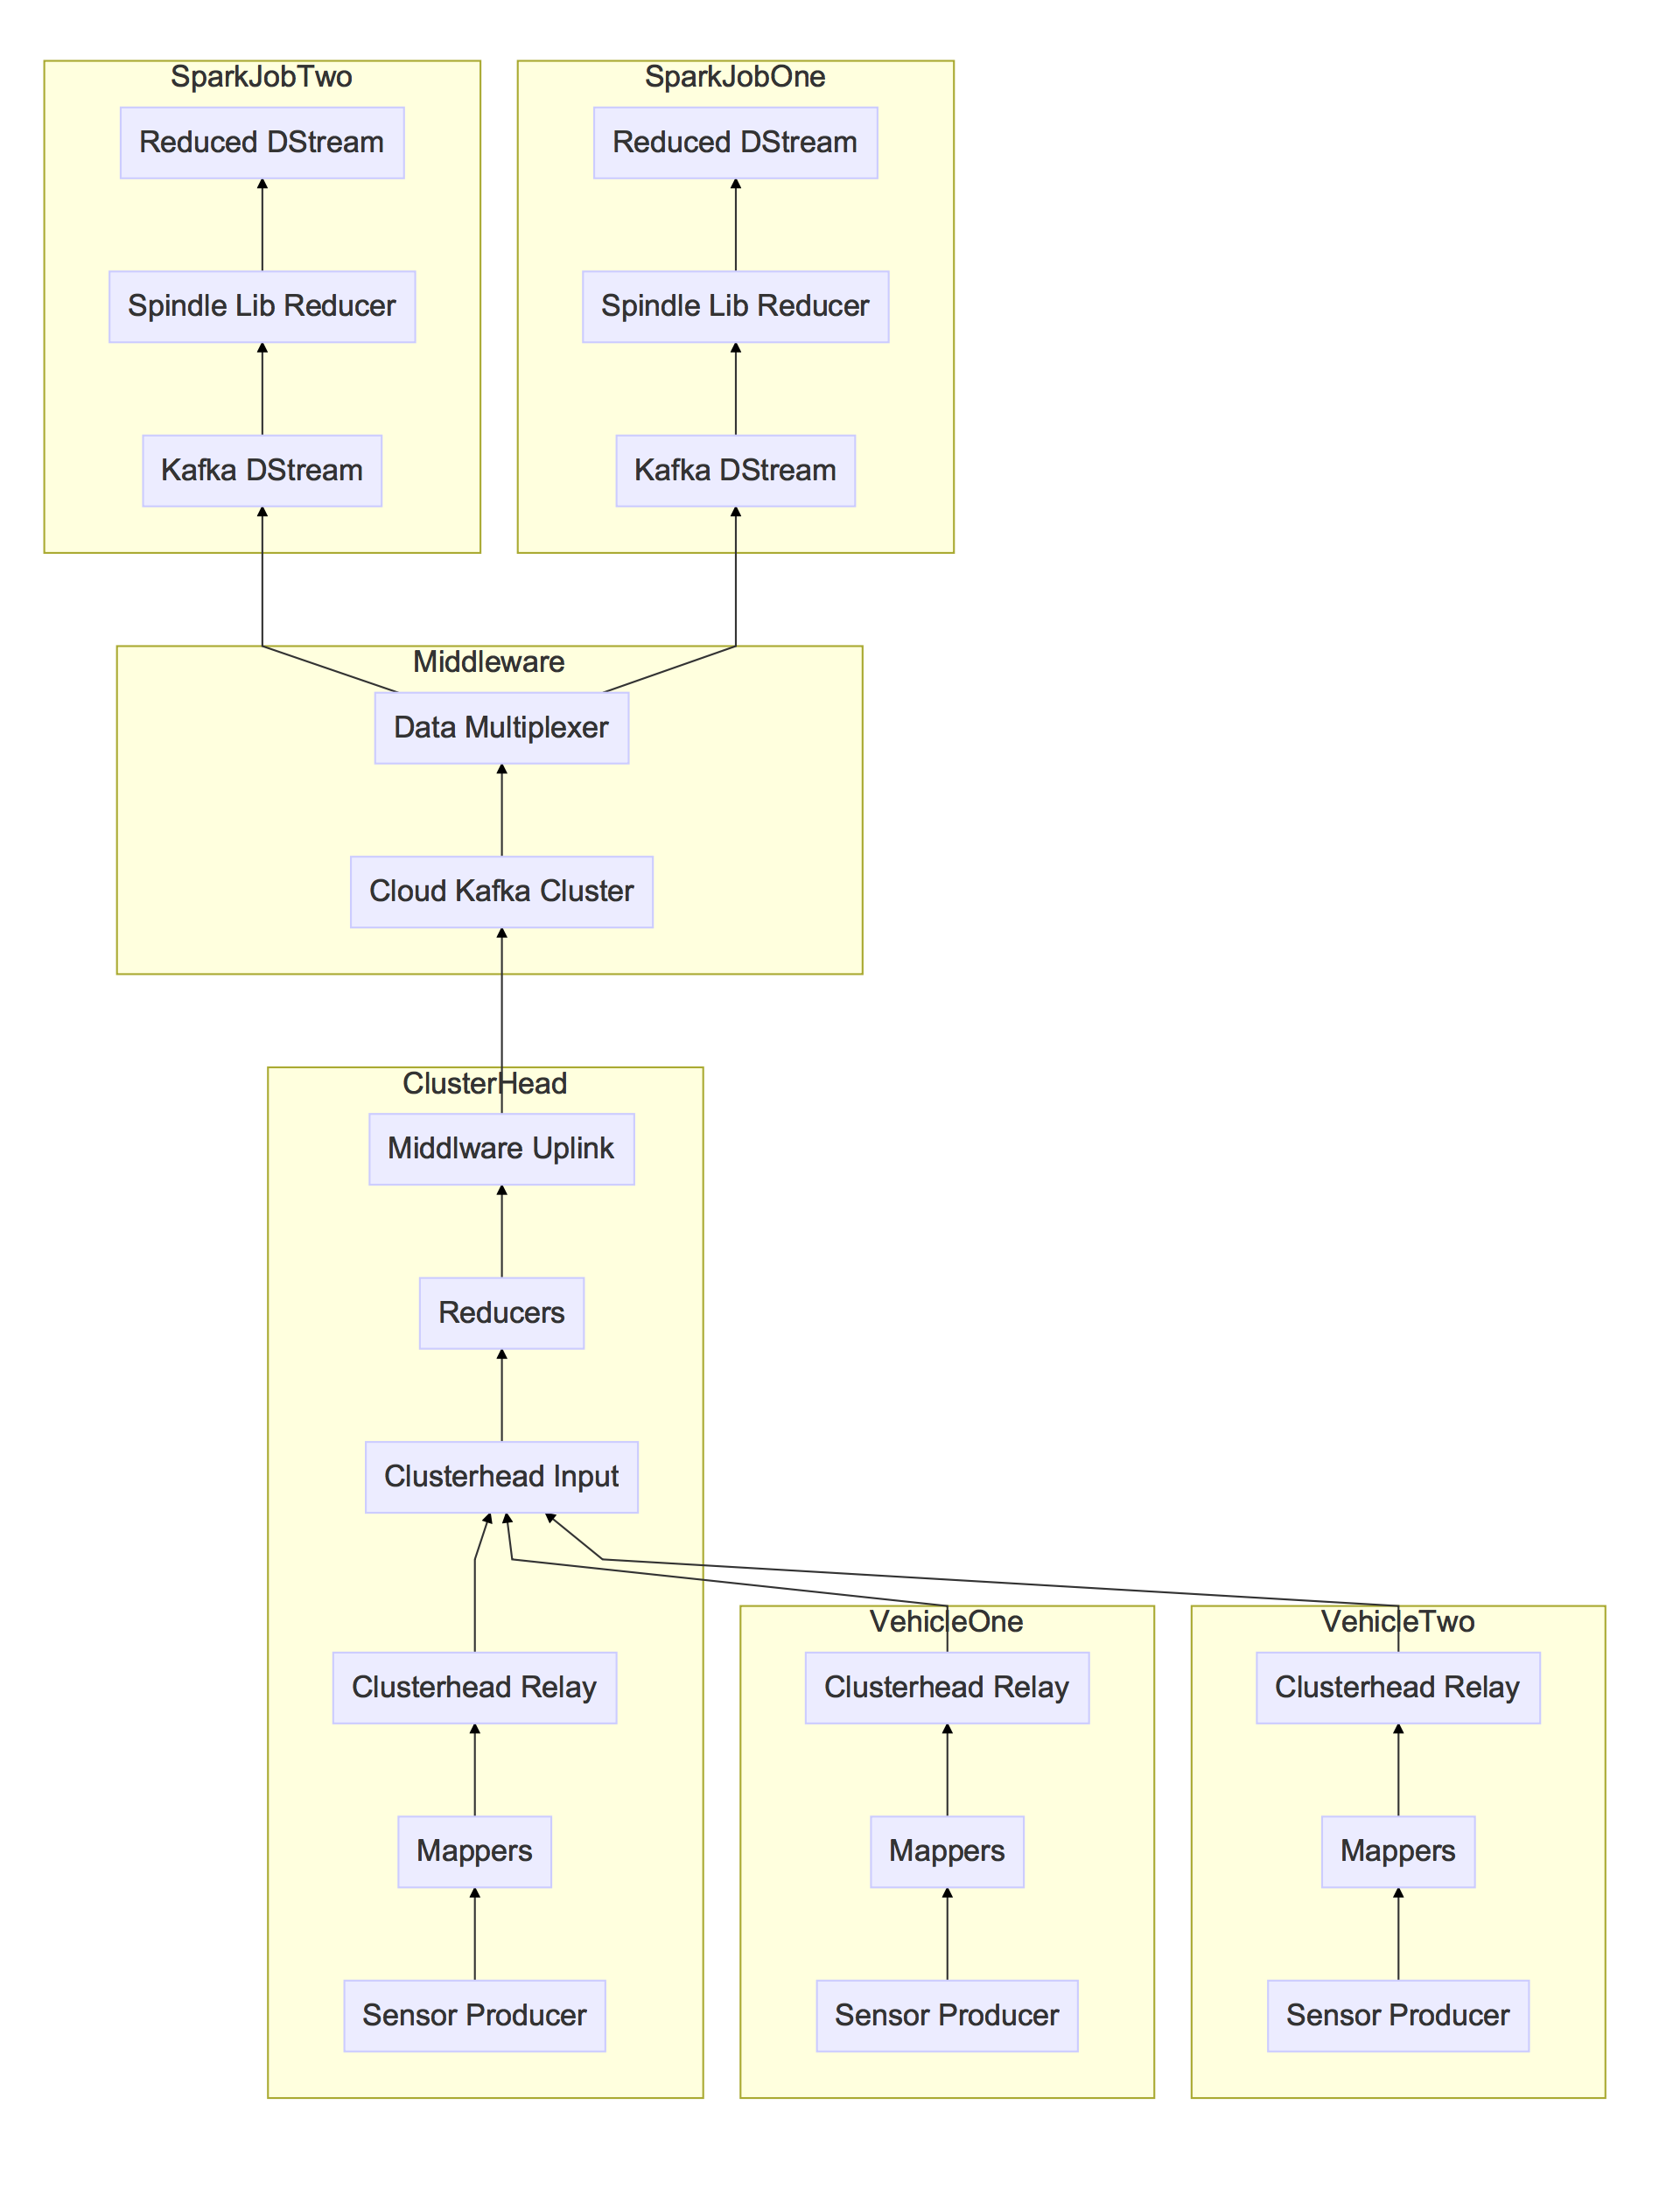
\includegraphics[width=0.5\linewidth]{binImages/theoretical-system.png}
        \caption{A diagram of the theorized system's major components. Vehicles
        send data to their Cluster Heads, which perform reduce operations over
        incoming mapped tuples. The resultant reduced tuples are then sent to
        the middleware to be distributed to the connected Spark jobs.}
        \label{fig:theoretical:component}
    \end{figure}
    \begin{figure}
        \centering
        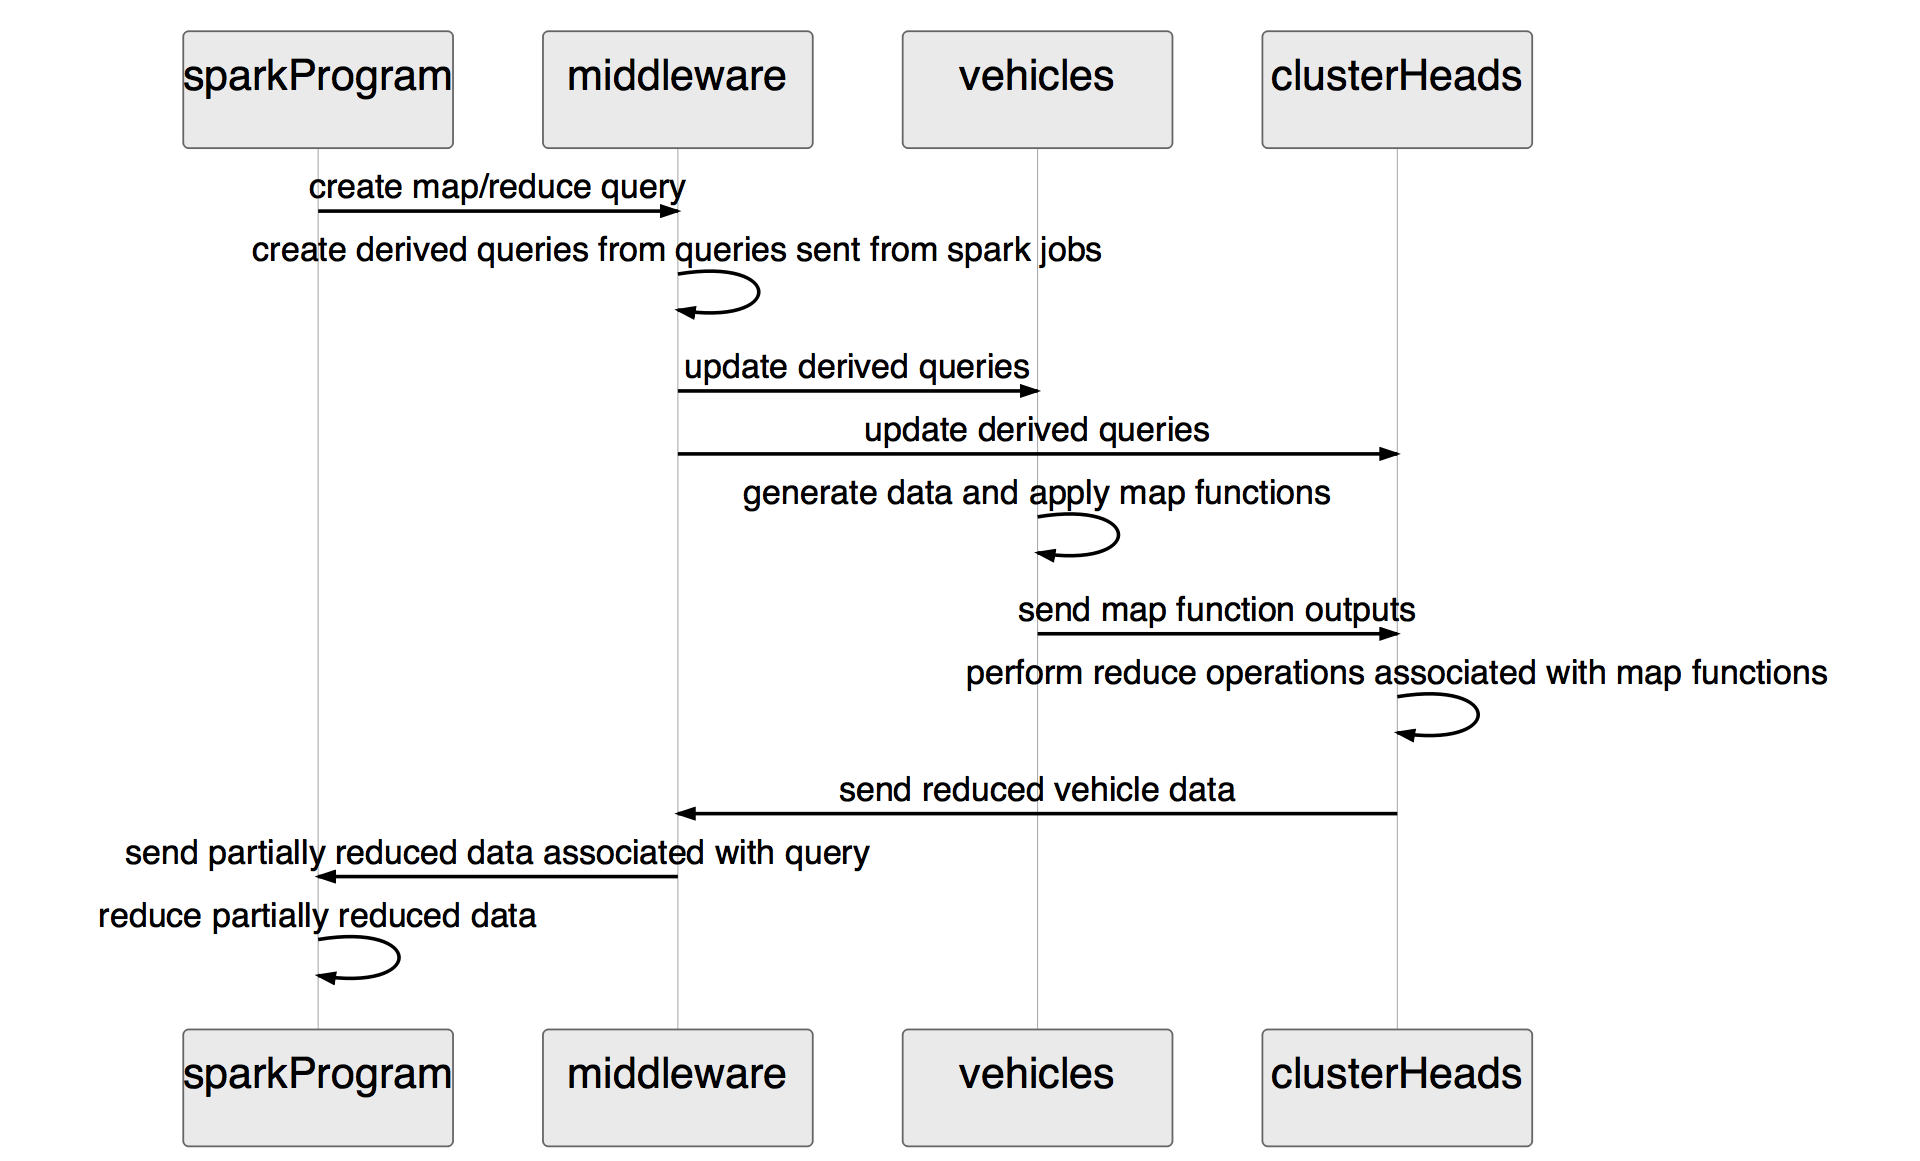
\includegraphics[height=4in, width=6in]{binImages/theoretical-sequence.png}
        \caption{A sequence diagram showing how a query passes from a connected Spark job
        through the middleware and vehicle systems and how the reduced results then return
        to the Spark job.}
        \label{fig:theoretical:sequence}
    \end{figure}

\subsection{Spark Clients}
    Spindle is ultimately designed to provide streaming data from network-connected vehicles to a streaming data
    analytics platform. We chose Apache Spark as our target platform. Apache Spark allows a user to analyze
    streams of tuples using the DStream programming abstraction previously described. In a traditional Spark
    Streaming program, a user creates a connection to some message bus such as Apache Kafka and programs against
    a DStream representing the micro-batches of messages being received from the connected message bus. The user
    is then free to analyze the data by applying functional transformations such as map, filter, and reduce
    to the batches of streamed tuples. 
    
    A naive analytics architecture for vehicle data with no edge computing optimizations
    would likely have each connected vehicle send all of its data directly over the internet to a message bus such as
    Apache Kafka running in the cloud. The user would then write a Spark Streaming program to create a DStream
    to receive the stream of all data coming from the vehicles and apply a map operation to extract only the 
    relevant values from the flood of incoming data. To perform an aggregate analysis of the data, the user would then
    apply a reduce operation, for example to get average fuel economy in real time for a given region or set of
    regions. While the naive example is extremely inefficient in terms of bandwidth consumption and compute resource
    utilization, the programming model is extremely simple and convenient. All the end-user writing the analysis
    has to do is connect, map, reduce, and output the results (or perform further analyses). 

    With the Spindle architecture, we attempt to preserve convenience of the naive model while greatly reducing
    bandwidth consumption and wasted cloud resources. To do so, Spindle includes a small Scala library that can be
    imported to a Spark Streaming program. Rather than calling the Kafka Spark Streaming library to create a 
    DStream, the user instead calls the Spindle Spark Streaming library to create their DStream. The user then
    writes their map and reduce functions as before, with the additional (current) requirement that the reduce function
    call be annotated with a descriptive enum to indicate the category of reduce operation taking place (e.g.\ min,
    max, mean, etc\dots).%TODO: reducebykey not reduce bah

    The Spindle Spark Streaming library is then able to serialize the user's map and reduce functions and transmit
    them to the middleware for de-duplication and distribution to vehicles and Clusterheads. The middleware
    sends back partially reduced results which the library running on Spark then re-runs the reduce function over.
    The final output is a DStream of reduced tuples, which from the user's perspective has the same attributes as 
    a DStream that would have been produced by running the naive implementation.

    We have developed a proof-of-concept implementation of the Spindle library for Spark Streaming described above.
    A future version will include the ability to pass filter functions to the middlware as well in order to support
    more selective queries.
\subsection{Middleware}
    Spindle's cloud middleware design consists of two components: a message bus and a query manager.
    \paragraph{Kafka Message Bus}
        Required vehicle data is published to a Kafka cluster, to which the Spindle Spark Streaming client can
        connect to consume partially reduced tuples for further processing as described above. Kafka provides
        a scalable platform with logical partitioning of messages (topics) that allows data from vehicle clusters
        for multiple Spark Clients to be ingested and routed to client-specific topics so that data for overlapping
        queries need only be sent once and so that each client can be required to process only the data required by
        its analysis.
    \paragraph{Query Manager}
        The query manager is responsible for storing, de-duplicating, and disseminating active Spark client queries.
        Duplicate map operations can be detected by their return types, while duplicate reducers can be detected
        by detecting duplicate inputs types, return types, and by their category annotations. Two queries can be
        de-duplicated if their mappers match, their reducers match, and their geographic regions overlap; if the
        geographic overlap is complete, then a single query is sent to the vehicles and clusterheads.
        As Kafka requires Zookeeper, a consistent distributed key/value store, the middleware will store its
        state and look for client queries in Zookeeper directories.
        Incoming data, from the cluster heads, will be loaded into Kafka. The query manager will then perform
        streaming map operations using Kafka Streams to route data to Kafka topics for the dependent queries.
        %SECONDPASS: flesh out how query manager works - describe how duplicate queries are not a problem, describe how messages are routed through kafka streams (by reducerIds)

\subsection{Vehicles and Clusterheads}
    The vehicles and Clusterheads run a similar software stack to that of the middleware, with data being
    processed through Kafka Streams. Each vehicle and Clusterhead is expected to have its own internal
    single-node Kafka cluster as well as supporting software for marshalling data, managing cluster membership,
    and applying map and reduce functions to the streaming data.
    Specific implementations of the protocols used to connected vehicles to one another, to clusterheads, and Clusterheads
    to the internet are beyond the scope of this work, as are the specifics of how best to propagate queries from the middleware
    query manager to vehicles and Clusterheads. Spindle's architecture requires only that vehicles be able to exchange binary
    data with clusterheads and that Clusterheads be able to send binary data to the cloud middleware. We anticipate that queries
    will be transmitted to vehicles by their Clusterheads, though a model in which vehicles periodically poll the cloud middleware
    directly is also compatible with the Spindle architecture.
    Every vehicle can act as a Clusterhead, though a Clusterhead need not be a vehicle and can instead be some other piece of
    connected infrastructure. The Spindle architecture is also agnostic to clustering algorithms and protocols, but merely requires
    that each vehicle know the identity of and be able to communicate with its Clusterhead (where the vehicle may be its own Clusterhead).
\subsubsection{Vehicle Components}
    \paragraph{Sensor Producer} 
        Each vehicle has a sensor producer, which is a Kafka message producer that periodically reads the current sensor data (e.g.\
        speedometer, tachometer, fuel consumption, fuel level, tire pressure, O2 sensors, lat/lon, etc\dots) and publishes the data
        as a single serialized VehicleMessage object to the onboard Kafka cluster. The VehicleMessage class is what the Spark client
        map functions take as input.
    \paragraph{Mappers}
        Each vehicle has a set of map functions loaded from the Middlewware. A local vehicle-level query manager periodically checks
        for updates to the set of active map functions. When a new map function arrives, the vehicle-level query manager
        launches a new Kafka Streams topology that reads data from the Sensor Producer topic, applies the map function to the 
        deserialized data, and publishes the serialized map function output to a dedicated output topic.
    \paragraph{Clusterhead Relay}
        Finally, each vehicle has a Clusterhead relay, which reads data from the mapper output topics and relays the data to
        the vehicle's current Clusterhead. This is where data is transmitted from vehicle to vehicle or vehicle to infrastructure
        over a wireless communication protocol. Spindle is protocol agnostic, as described above.
\subsubsection{Clusterhead Components}
    \paragraph{Clusterhead Input}
        The Clusterhead Input is a Kafka producer, which receives messages transmitted by the member vehicle
        Clusterhead Relays and publishes the messages to a single local Kafka topic.
    \paragraph{Reducers}
        Just as on the vehicles, the Clusterheads have a local query manager which is responsible for loading and unloading
        query functions. Instead of loading and unloading map functions, the Clusterhead query manager loads and unloads
        reduce functions. Once again, the reduce functions run on Kafka Streams topologies, with the distinction that the
        reducer topologies include buffers, which cache intermediate reduce results until some pre-defined time window
        has passed, at which point the reduced data for a time window is published to a Middleware Uplink Kafka topic.
    \paragraph{Middleware Uplink}
        The Middleware Uplink serves a similar purpose to that of the vehicle's Clusterhead Relay. The uplink
        reads messages published to the Middleware Uplink Kafka topic and sends the messages to the cloud Middleware.
        It is at the Middleware Uplink that message compression and de-duplication can occur. If two reducers produce
        the same output in a given time window, the Middleware Uplink should send only one tuple, tagged with the UIDs
        of both reducers. %SECONDPASS: go into more detail about deduplication (walk through a scenario, possibly write a new subsection)


%GENERAL NOTE: need to be able to understand what the figure is solely through the caption (fine to duplicate text)
    %TODO: walk through spark query, middleware update, propagation through vehicle networks, vehicle-level-map, clusterhead-reduce, transmission to middleware, transmission to spark streaming, secondary reduce, etc..

    %TODO(meeting): do simple physical layout diagram

\section{Simulation Architecture}
    We have developed a simulator to evaluate the vehicle and Clusterhead architecture under a variety of clustering,
    vehicle density, and query configurations.

    The simulator implements the basic features of the vehicle and Clusterhead software described above, including
    Sensor producers, mappers, reducers, simulated Clusterhead relays, query managers, and simulated middleware uplinks.
    The core simulation software is implemented in Scala using the Akka actor framework.
    %SECONDPASS: do a system diagram for the simulator
    \begin{landscape}
        \begin{figure}
            \centering
            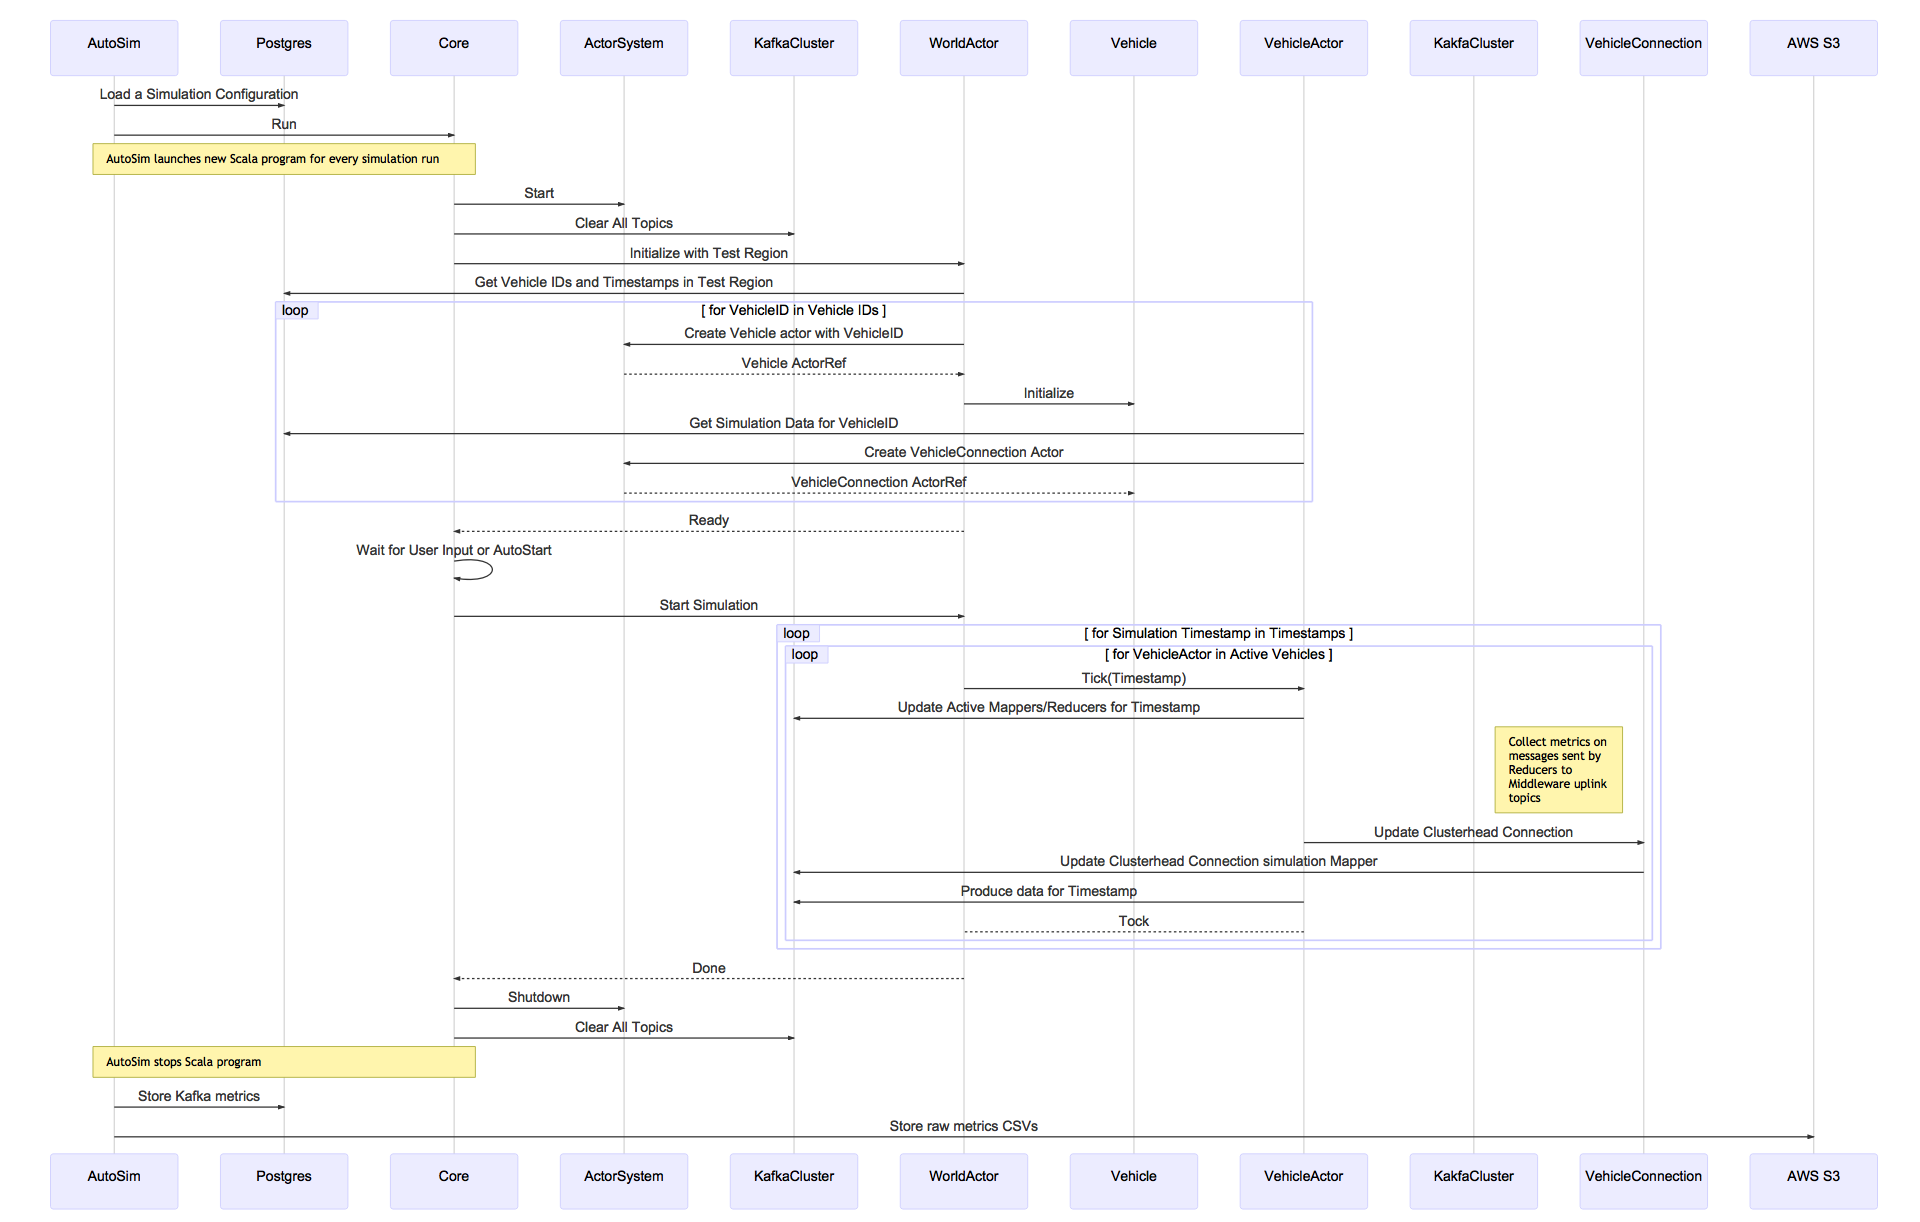
\includegraphics[width=\textwidth]{binImages/simulator-sequence.png}
            %TODO (meeting): increase font size and increase size of figure to be as large as will fit in margin
            \caption{A sequence diagram showing the high-level interactions of
            the Spindle simulator components. A Postgres database stores the
            simulation configurations and pre-computed velocity and connectivity
            data, as well as simulation results.}
        \end{figure}
    \end{landscape}

\subsection{SpindleSim}
    The Spindle simulator (SpindleSim) is implemented in several thousand lines of Scala \cite{scala} 
    and is implemented on top of the Akka
    actor model framework. The Scala/Akka portions of the simulator implement as realistically
    as is practical the software that would run on a real-world deployment of Spindle. This is
    accomplished by creating a separate Akka actor for each simulated vehicle, where each actor
    is given a cache of time-series simulation events and data and a connection to a ``World''
    actor responsible for keeping track of global simulation time; this global time-keeper 
    can be thought of as a stand-in for a GPS clock running on each vehicle. Each vehicle
    actor is then responsible for managing its publish-subscribe streams and messages, as well
    as its simulated connections to other vehicles in its cluster. Messages are exchanged between
    vehicles and send from vehicles to ``the cloud" by way of special "Stream Relay" Kakfa Streams
    programs. The Stream Relay programs operate as simulated versions of the Clusterhead Relay
    and Middleware Uplink programs. Stream Relays are also responsible for filtering 
    expired and "Canary" messages; the verison of Kakfa Streams being used (the latest version
    at the start of development) has implementation bugs that mean new message consumers must
    read old messages and that a topic may not fully initialize until a message is produced to it;
    our solution is to send "Canary" messages to ensure topic initialization and to filter out messages
    that have already been processed. Finally Stream Relays are responsible for keeping a 
    running sum of the number of bytes sent on a per-relay basis and logging these sums to separate 
    CSV files at run-time.
\subsection{AutoSim}
    The Scala/Akka simulator (SpindleSim) currently has a number of pre-configured map/reduce jobs written
    that can be turned on or off using the program's \verb|application.conf| file. A secondary
    program, dubbed AutoSim, runs the simulator iteratively, writing to the conf file, launching
    SpindleSim, then gathering the results and uploading them to a database and permanent storage.
    In order to iterate through the desired test configurations, AutoSim reads from a table \verb|sim_configs_vx| in a 
    Postgres 9.6.1 database hosted on an AWS EC2 \verb|m4.large| reserved instance.
    AutoSim will choose among the least-tested configurations in the configs table, write the configuration to
    the SpindleSim \verb|application.conf|, and launch an instance of SpindleSim. While SpindleSim is running, AutoSim
    greps the console logs for exception messages. If an exception is detected, the current SpindleSim instance is killed
    and a notification is sent via AWS SNS topic reporting the error message in order to facilitate debugging. If the SpindleSim
    operation completes, AutoSim uploads the CSV logs to an AWS S3 bucket and parses the final message byte sums from the CSV
    files then writes the results to a \verb|sim_results_vx| table in Postgres. AutoSim is a simple Node.JS ES6 application
    that is run from the Babel-Node \cite{babel} transpiler.
% Focus more on envisioned 
% Follow Cloud Computing papers for format (upper bound on page count is 5-10 pages)

%separate sections for envisioned architecture and for test design ("accommodations for testing")
    %TODO(meeting): describe mapping of theorized system onto simulator

\chapter{Experiments}
\section{Data Sets}
\subsection{Vehicle Traces}
   The Spindle experiments depend on a set of vehicle traces 
   generated using "the open source vehicular network simulation framework" VEINS, which simulates
   vehicle movement and radio connectivity in a "realistic" manner \cite{veins}. The VEINS traces
   were generated by Mike Wittie of the Montana State University as part of a larger overall research
   project. 
   The traces come in the form of sharded CSV files containing time-series mappings of three different types:
   speed, x-position, y-position, and connectivity to other vehicles. Each time-series mapping includes
   a timestamp, a vehicle uid, and a value (speed, position, reachable-vehicle-id). 
   These shards have been parsed into a Postgres database with a table for each mapping type.
   %TODO(MEETING): insert information about City of Cologne
   % insert information about node count, length of time here
   % Saw we pick sparse, dense region, etc... here (move from subsection below)
\subsubsection{Test Regions} %TODO(MEETING): make sub-sub section of Vehicle traces subsection
    \paragraph{Original VEINS Traces}
        The original VEINS traces span a region from $(41735, 85178.4)$ to $(63071.5, 114426)$ and includes 3340 distinct
        vehicles. This dataset includes more vehicles than the current simulator implementation can handle due to the large
        number of threads, network connections, and Kakfa topics that would be required (the thread/topic count scales with the
        number of vehicles multiplied by a constant multiple of the average number of map/reduce queries running on each node).
        A real-world deployment would distribute the threads/topics over the set of vehicles in the system such that each
        vehicle and kafka cluster would have threads and topics proportional to the number of active map/reduce queries.
        In essence, this is a temporary limitation of the simulation architecture, not the real-world architecture.

        To overcome the simulator's limitations, we defined two test regions, one dense region and one sparse region
        being transited by approximately the same number of vehicles. The sparse and dense regions were selected based
        on the number of vehicles transiting them and based on the layout of the underlying road networks.

    \begin{figure}
        \centering
        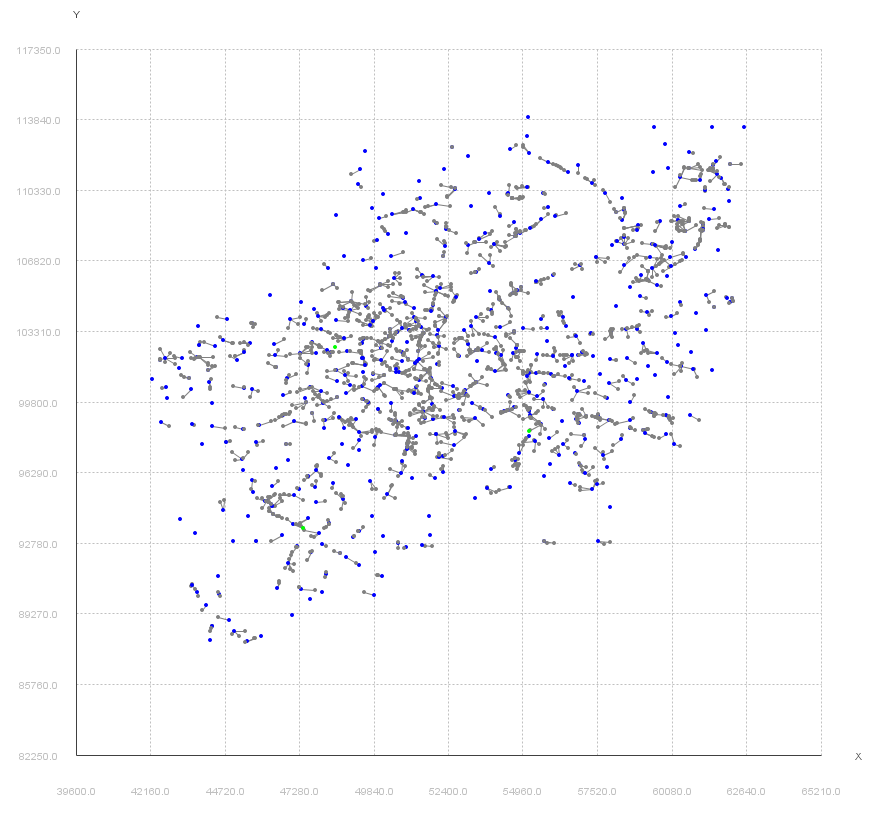
\includegraphics[scale=.5]{binImages/xiaotian-clusters.png}
        \caption{Illustration of VEINS Vehicles with MANET Clustering, Courtesy Xiaotian Duan}
        \label{fig:clusters}
    \end{figure}
    \begin{figure}
        \centering
        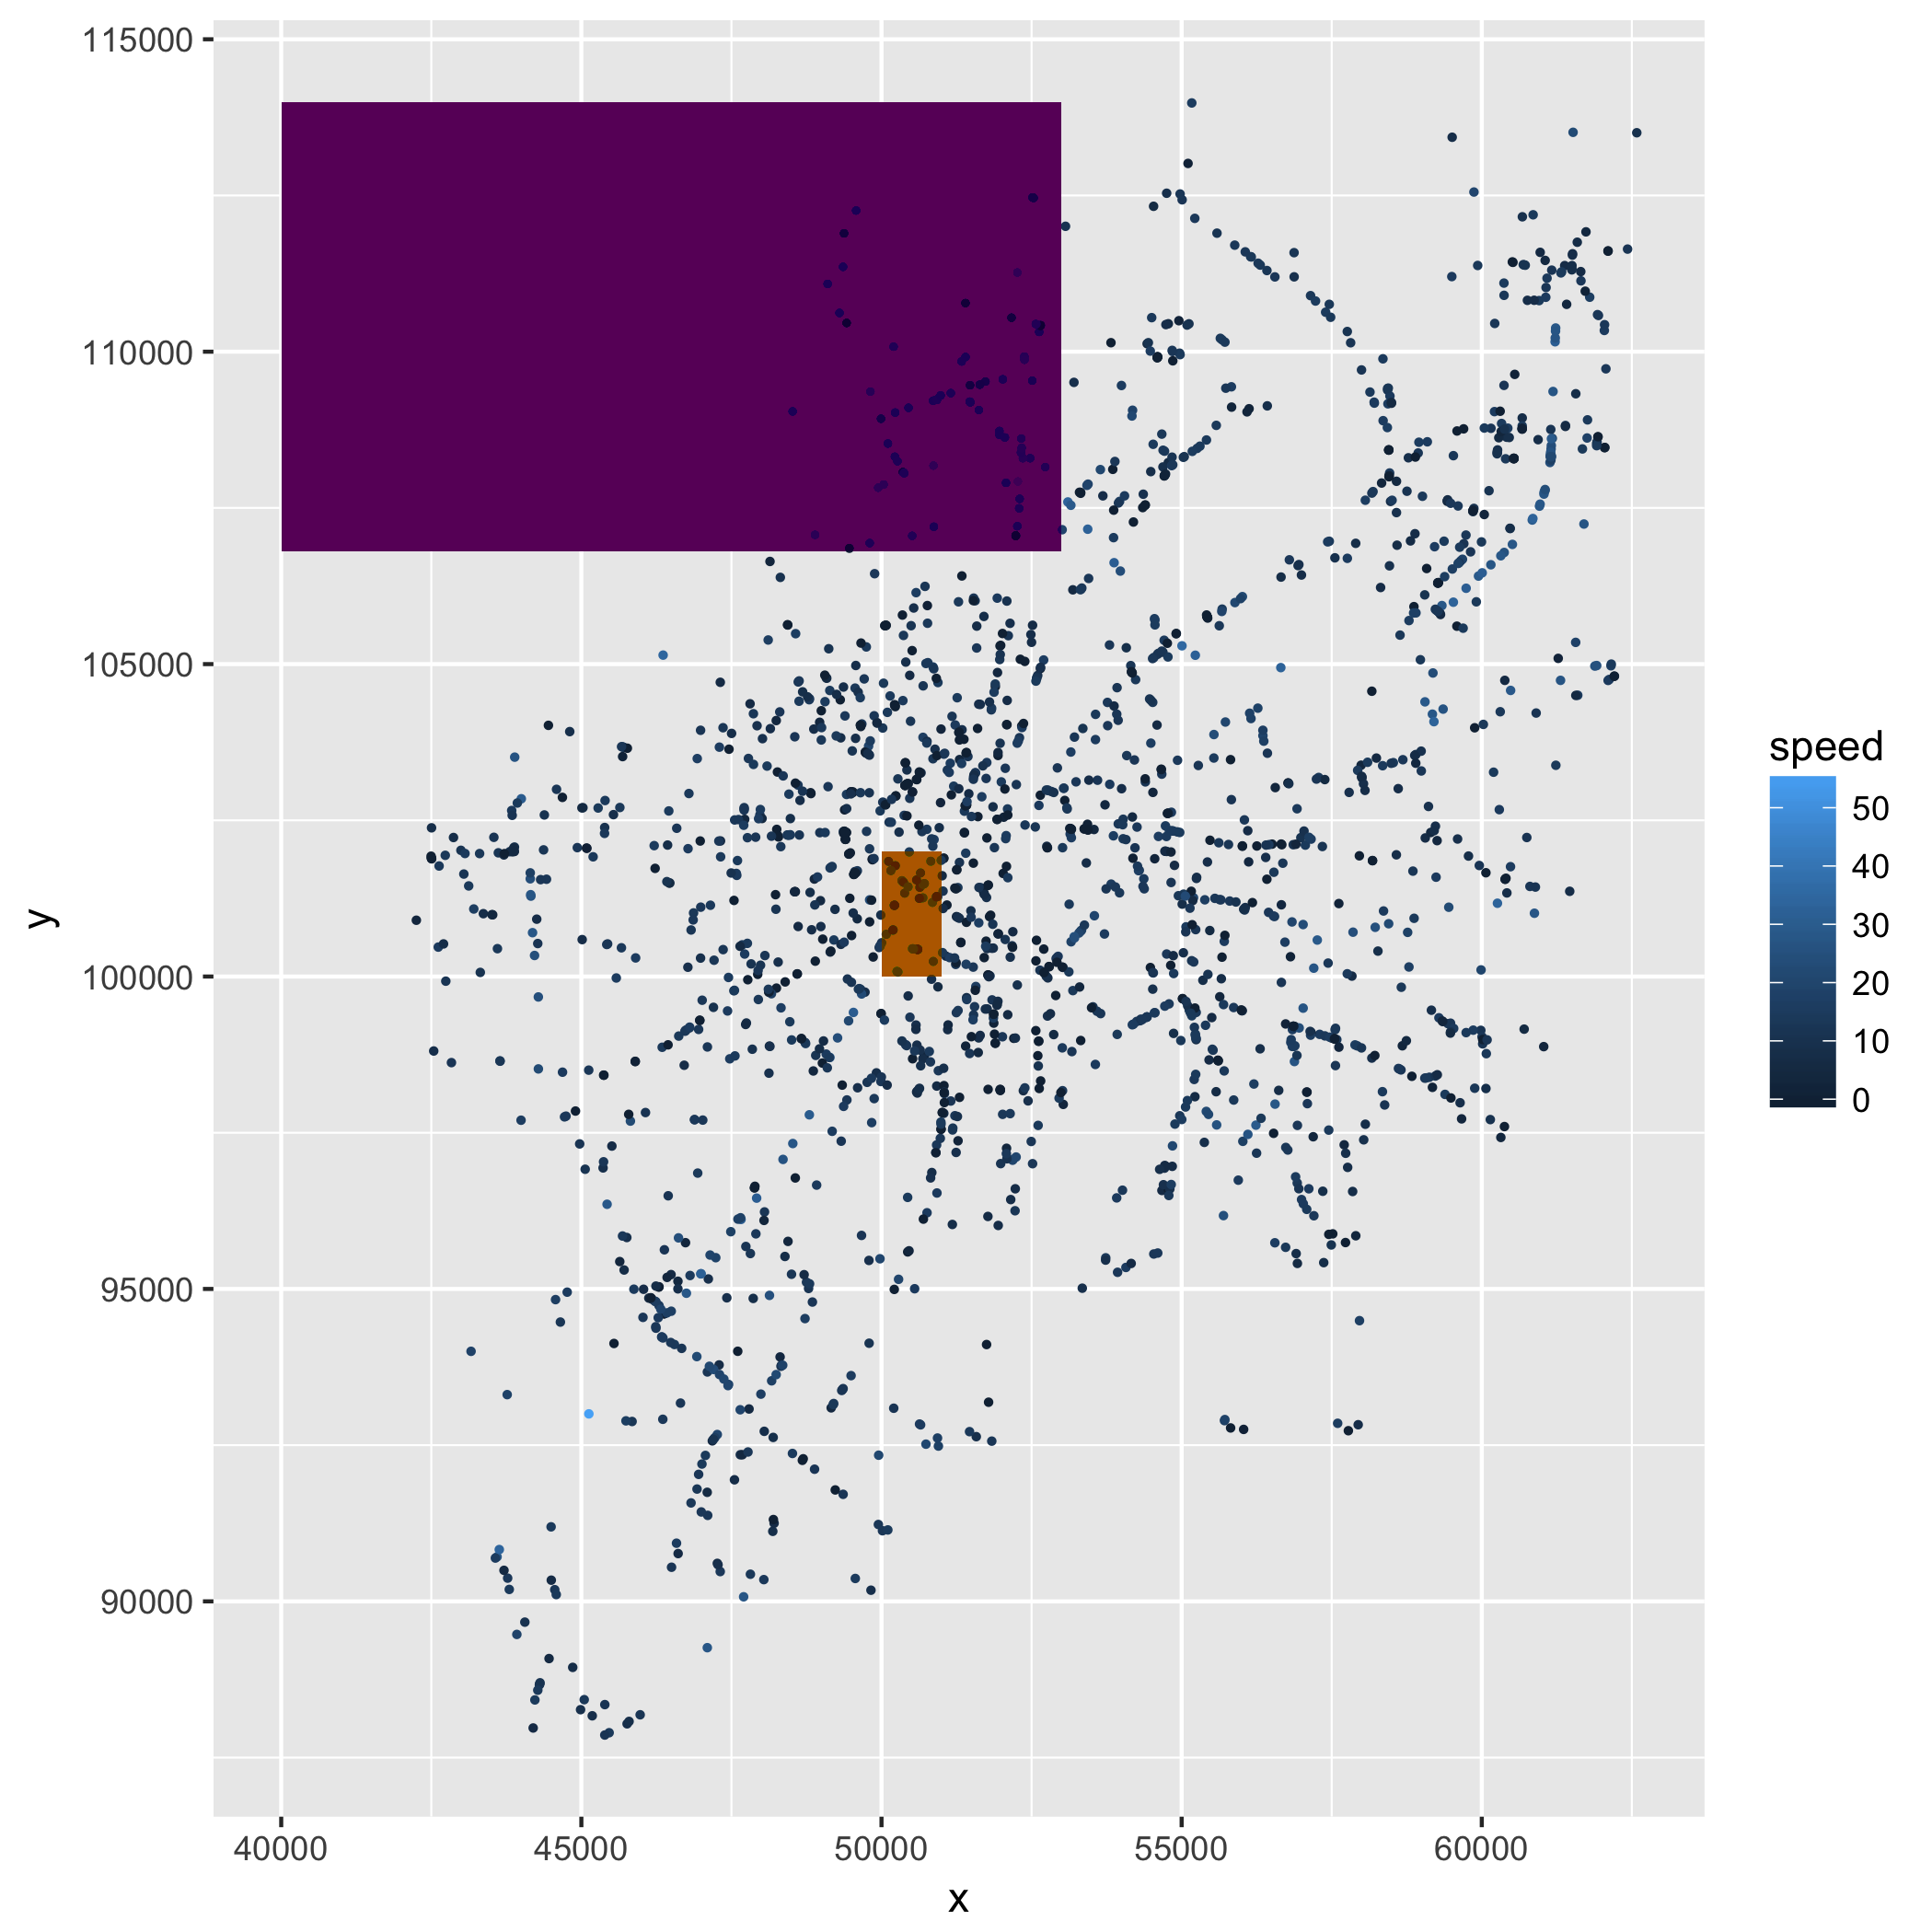
\includegraphics[scale=.2]{binImages/cars.png}
        \caption{A Snapshot of Active Vehicles in VEINS Traces with Selected Regions Highlighted}
        \label{fig:regions}
    \end{figure}
    \paragraph{Sparse Region}
        The sparse region is transited by 148 distinct vehicles over the course of the simulation and defines a bounding
        box from $(40000, 106800)$ to $(53000, 114000)$. The sparse region covers an area on the outskirts of the city,
        with a relatively low density of vehicles. The sparse region is illustrated by a purple box in \ref{fig:regions}.
    \paragraph{Dense Region}
        The dense region defines a bounding box from $(50000, 100000)$ to $(51000, 102000)$ and is transitied by
        131 vehicles over the course of the simulation. The dense region covers a small area near the city center
        where the density of vehicles is higher. The dense region is illustrated by an orange box in \ref{fig:regions}.

\subsection{Window Sizes}
    Kafka Streams can perform reduce operations over messages received over the course of a user-defined time-window
    and will write the results to a KTable, a logical structure whose API approximates that of a key-value store. %TODO: citations
    Spindle's Kafka Streams reducer adds a \verb|Batcher|, which transmits the final value of a time-window's KTable
    entry to some destination Kafka topic (in this case the middleware). As such, Spindle supports micro-batch operations
    on Kafka streams with user-configurable window sizes. The sizes tested were 10, 15, and 30 seconds.
\subsection{Test Clusters}
    The cluster head assignments for each node are pre-computed using either Xiaotian's %TODO: cite Xiaotian
    clustering algorithm or some base-line \verb|single_clusterhead| (all vehicles in simulation share a single clusterhead)
    or \verb|self_clusters| (all vehicles act as their own cluster heads).
\subsection{Clustering Algorithms}
    The spindle architecture takes advantage of work done by fellow RPI student Xiaotian Duan on generating
    clusters of vehicles based on vehicle connectivity and lane position. 
    %TODO: get permission from Xiaotian for using clustering images
    %TODO: include information about cluster density for each clustering (sparse/dense)
    %TODO: Fix the quotes!

\section{Test Software Environment}
    AutoSim and SpindleSim are packaged inside a docker image, \\\verb|wkronmiller/nsl-spindle-simulator| that can be run from
    a laptop, desktop, or EC2 instance. The test framework and container are designed to survive the total loss of local
    storage and/or the running simulator container by storing the results of all completed simiulation operations on
    S3 and a remote database. This design decision allows the test framework to be run on an AWS EC2 Spot Fleet %TODO: citation
    which offers discounts of roughly 70-90\% in exchange for the requirement that any software running on a Spot instance
    be designed to killed at any time with little or no warning. %TODO citation
    The architecture also enables trivial transfer of the simulator across different machines, easing debugging and mitigating
    problems related to transient EC2 network problems. 

\section{Test Configurations}
\subsection{Example Map/Reduce Programs}
    \paragraph{speedSum}
        The most simple map/reduce operation tested is the "speedSum" job, which simply takes the sum of the speeds of all
        vehicles in the simulation in each time step. The map operation takes the vehicle state as input and returns only
        the vehicle speed. The reduce operation run at the clusterheads takes the sum of the speeds
        of each of the cluster member vehicles.
    \paragraph{geoFiltered}
        The geoFiltered operation collects the data required to compute the average speed of all vehicles in a selected
        geographic region. This map/reduce job extends speedSum by performing a word-count-style map operation that maps each vehicle's sensors
        to the vehicle count and the vehicle speed: \verb|(1, [speed])|. The reduce operation again simply sums the count
        and speed of each member vehicle \verb|([numVehiclesInCluster], [sumOfSpeeds])|. The geoFiltered query also is selective,
        in that for a given test region the geoFiltered query operates only on a subset of the test region containing approximately
        half of the vehicles being tested.
    \paragraph{geoMapped}
        The geoMapped query performs a similar map/reduce operation to geoFiltered, but instead of filtering out half the
        test region, the geoMapped query maps half the test region to one region ID and maps the other half of the
        test region to a second region ID, then performs a reducebykey. The map operation produces the following:
        \verb|(regionId) -> (1, [speed])| and the reduce produces \verb|(regionId) -> ([numVehiclesInCluster], [sumOfSpeeds])|.

\section{Simulator Results}

   A total of 114 trials were carried out for the geoMapped query and a totla of 111 trials for speesSum.
   Figures \ref{results:speedsum} and \ref{results:geomapped} show the bandwidth consumed by the speedSum
   and geoMapped map/reduce queries, respectively. We see from both sets of graphs the same pattern: that
   the higher density region has better performance than the lower density region, that larger window
   sizes have better performance than smaller window sizes, and that, critically, the use of clustering
   results in a 50-75\% savings in bandwidth.

    \begin{figure}
        \centering
        \begin{subfigure}[h]{0.45\textwidth}
            \centering
            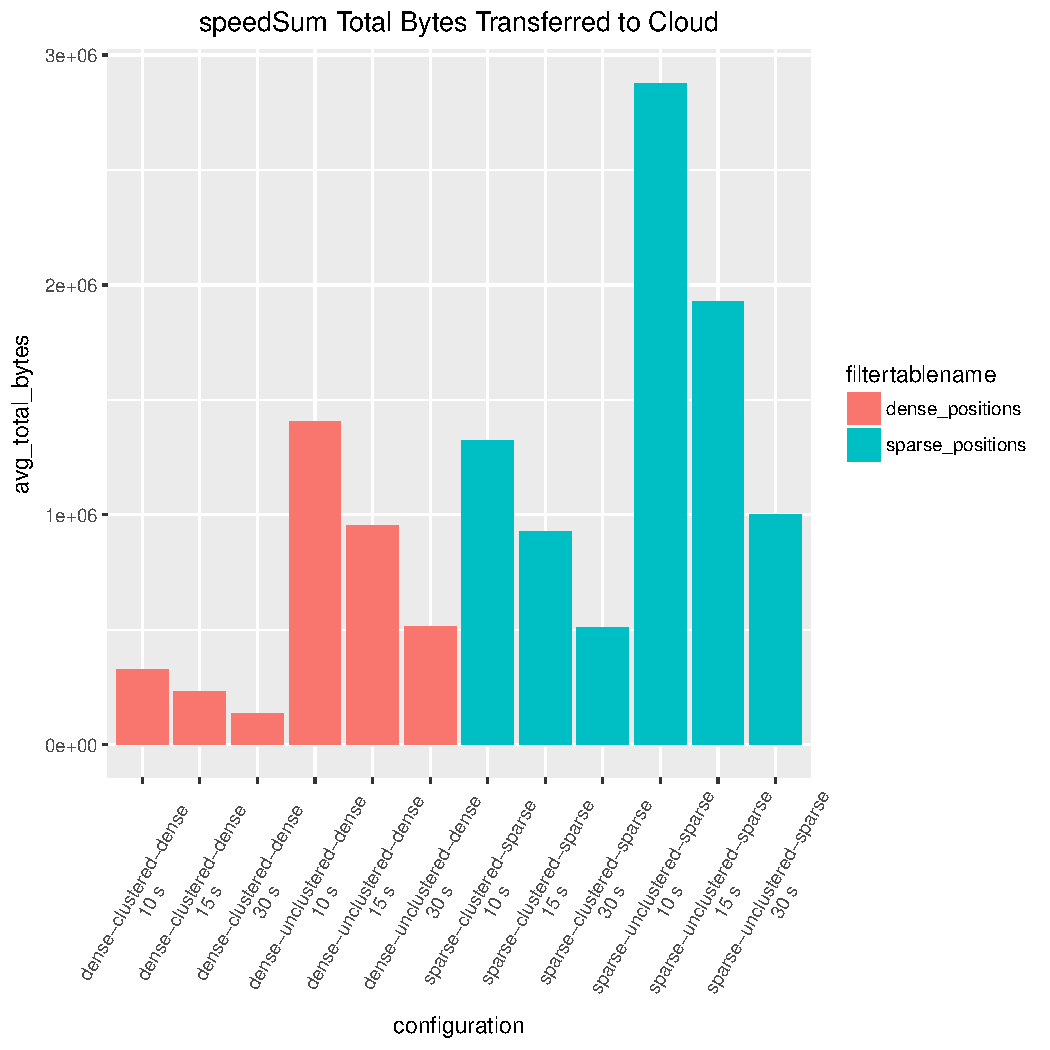
\includegraphics[width=\textwidth]{binImages/speedSum-runplot.pdf}
            %NOTE (Meeting)
            \caption{The total number of bytes sent to the middleware,
            averaged over multiple trials for the speedSum map/reduce job.} 
        \end{subfigure}
        \begin{subfigure}[h]{0.45\textwidth}
            \centering
            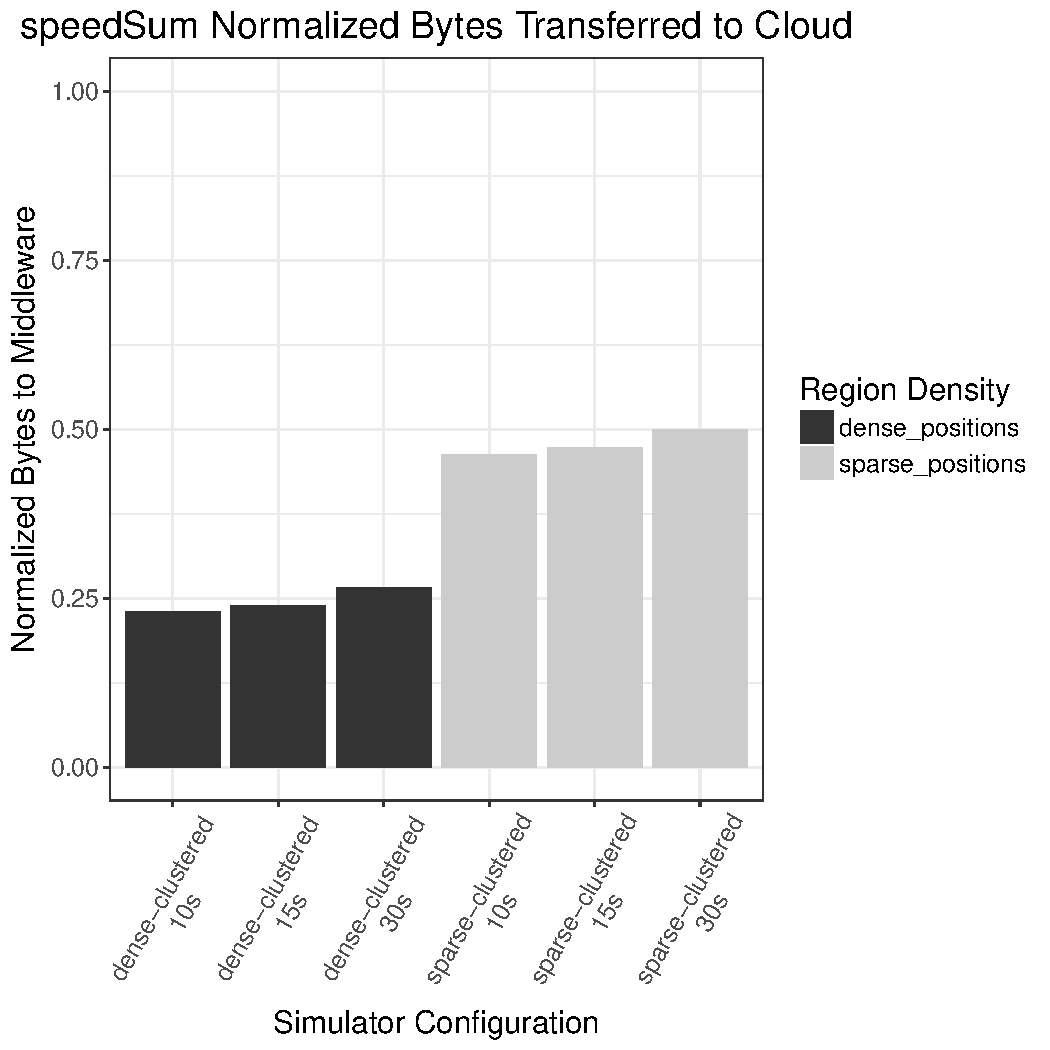
\includegraphics[width=\textwidth]{binImages/speedSum-runplot-normalized.pdf}
            \caption{The scaled number of bytes sent to the middleware in a given region and window size
            configuration where y=1 indicates the number of bytes sent without clustering for a given region
            and reduce window size.}
        \end{subfigure}
        \caption{Results from running the speedSum map/reduce query. The x-axis contians different
            configurations of regions, clusterings, and reduce window sizes (10, 15, and 30 seconds). Smaller
            values in the same geographic region indicate better performance, where the best performance
            comes from using clustering with a 30 second window size. Demonstrates the data savings that occur as a result of using
            vehicle clusters. Also illustrates how data reduction is affected by regional vehicle
            density - areas of high vehicle density can take better advantage of clustering to get more savings.}
        \label{results:speedsum}
    \end{figure}
    \begin{figure}
        \begin{subfigure}[h]{0.45\textwidth}
            \centering
            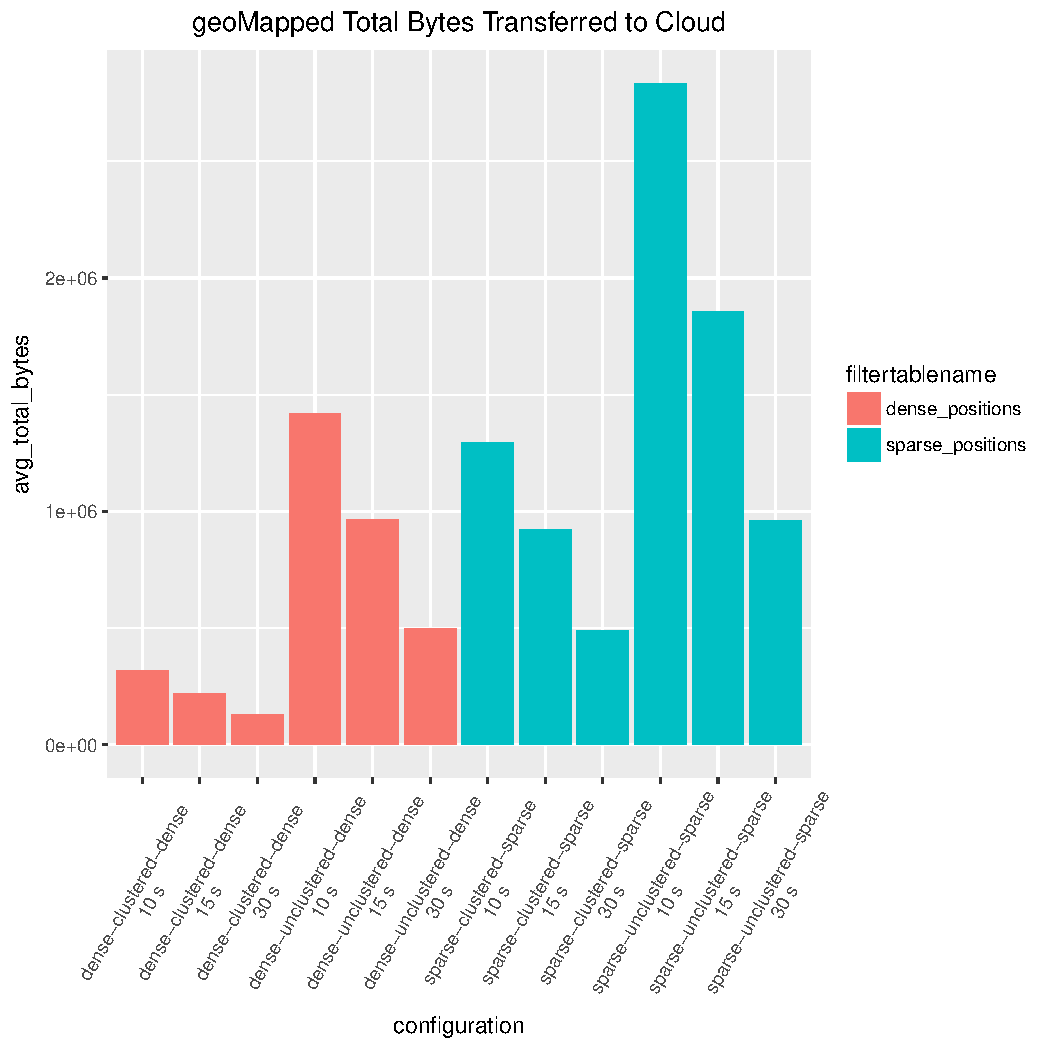
\includegraphics[width=\textwidth]{binImages/geoMapped-runplot.pdf}
            \caption{The total number of bytes sent to the middleware,
            averaged over multiple trials for the geoMapped map/reduce job.}
        \end{subfigure}
        \begin{subfigure}[h]{0.45\textwidth}
            \centering
            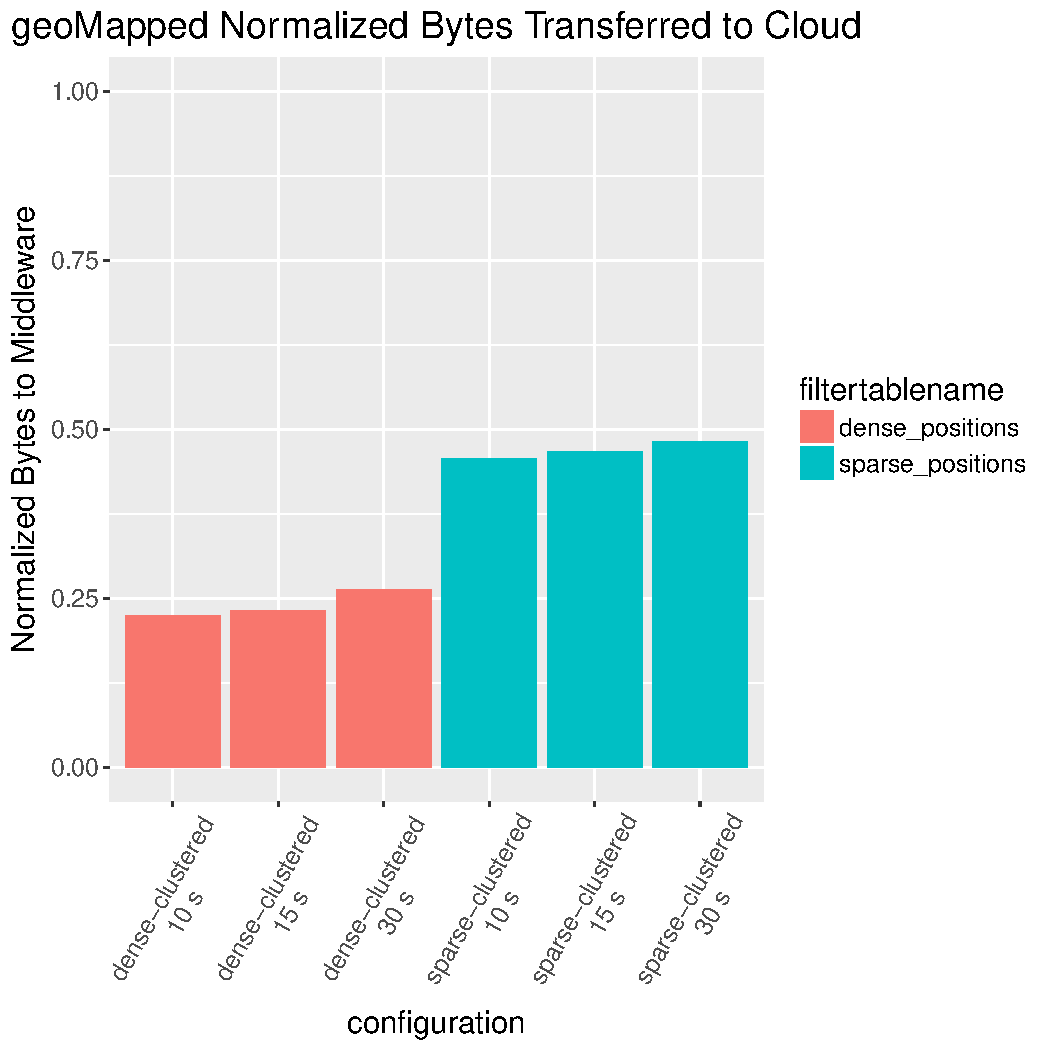
\includegraphics[width=\textwidth]{binImages/geoMapped-runplot-normalized.pdf}
            \caption{shows the scaled number of bytes sent to the middleware in a given region and window size
            configuration where y=1 indicates the number of bytes sent without clustering for a given region
            and reduce window size.}
        \end{subfigure}
        \caption{Results from running the geoMapped map/reduce query. The x-axis contians different
            configurations of regions, clusterings, and reduce window sizes (10, 15, and 30 seconds). Smaller
            values in the same geographic region indicate better performance, where the best performance
            comes from using clustering with a 30 second window size. Demonstrates the data savings that occur as a result of using
            vehicle clusters. Also illustrates how data reduction is affected by regional vehicle
            density - areas of high vehicle density can take better advantage of clustering to get more savings.}
        \label{results:geomapped}
    \end{figure}

    The results make logical sense. A higher density region allows for better clustering - more vehicles to a cluster.
    A larger window size results in a smaller number of transmissions from the reducers to the middleware, so even
    though the serialized messages may be larger (because the values contained within are larger), the larger message
    size is outweighed by the lower transmision frequency; this makes sense when one considers the inevitable boilerplate
    required in each message that gets wrapped around the changing values. Finally, the use of clusters makes sense for
    similar reasons to those of having larger window sizes - fewer overall messages are sent.
    %SECONDPASS: table of results

\chapter{Conclusion}
    In this paper, we discuss the state of the art in connected vehicle technologies as well as the problem
    of managing the vast quantities of data these vehicles are expected to produce. We further discuss
    some of the use cases that are being explored for the wealth of information that researchers expect
    to be available in these new connected cars. Finally, we review current and upcoming cloud technologies
    related to data processing, particularly with respect to the Internet of Things. Next, we provide an
    overview of a novel solution to the problem of managing vehicle data by extending cloud and big data 
    technologies such as the map/reduce paradigm and Apache Kafka to the edge using the Spindle architecture.
    We discuss how existing tools such as Apache Spark can interfaced with edge computing systems through
    the use of the Spindle library for Spark Streaming.

    We demonstrate the power of our paradigm by creating a simulator for our vehicle and Clusterhead software,
    which we test under a number of different workloads. We then demonstrate that the combination of clustering
    and message reduction used in our architecture produces significant bandwidth savings.

\section{Future Work}
    In this work, we have demonstrated the efficacy of the core of the Spindle architecture - dynamic map/reduce
    on vehicles. There are a number of directions for future work, including extensions to the simulator and, 
    more critically, extensions to the architecture.
    It should be possible in the future to implement a full-stack simulator that launches spark clients, runs
    the cloud middleware, and interfaces with the existing SpindleSim software. We also believe it is worth
    investigating what other functions can be run at the edge, such as join and group functions, as well
    as how multiple simultaneous queries with such functions can be optimized to minimize the duplication
    of messages. By developing a more rich edge computation system, it will be possible to run more sophisticated
    algorithms at the edge, for example with the addition of stateful operators it might be possible to run
    machine learning algorithms at the vehicle and Clusterhead level.
    %SECONDPASS: give a concrete example of a machine learning algorithm

    Beyond tweaking Spindle, itself, we believe there is now an opportunity for further research that builds
    upon the framework. Particularly, there are opportunities for improvements to vehicle clustering algorithms
    to improve cluster size and stability by integrating available information. Furthermore, the topic of what
    useful information can be gathered from connected vehicles will likely remain a perpetually open question,
    now that it is possible to combine sensor and traffic information with other online data sources; we saw
    how one group combined the data with geographic information, but there may be other interesting datasets
    to pull in - everything from data on road construction to public event lists to economic data could be
    correlated with traffic flows. Furthermore, as has is being addressed in other research projects %TODO: cite a reference
    vehicles are themselves rich sensor platforms that can be used for gathering environmental data; it must
    now be determined what data is worth storing and to what degree of granularity it should be kept.
    %SECONDPASS: more ideas please

\specialhead{LITERATURE CITED}
\begin{singlespace}
\bibliographystyle{acm}
\bibliography{rpithes-short}
\end{singlespace}
\end{document}
